\documentclass{beamer}

\usetheme{Boadilla}
%\usetheme{Pittsburgh}
\usecolortheme{beaver}

\setbeamercovered{transparent}
\setbeamertemplate{navigation symbols}{} %remove navigation symbols

\usepackage[english]{babel}
\usepackage[latin1]{inputenc}

\usepackage{times}
\usepackage[T1]{fontenc}

\usepackage{animate}

% see http://tex.stackexchange.com/questions/86188/labelling-with-arrows-in-an-automated-way
\usepackage{tikz,amsmath,verbatim}

\newif\ifclipme\clipmetrue
\tikzset{labelstyle/.style={LabelStyle/.append style={#1}},linestyle/.style={LineStyle/.append style={#1}}}
\tikzset{LabelStyle/.initial={},LineStyle/.initial={}}

\newcommand{\mathWithDescription}[4][]{{%
    \tikzset{#1}%
    \tikz[baseline]{
        \node[draw=red,rounded corners,anchor=base] (m#4) {$\displaystyle#2$};
        \ifclipme\begin{pgfinterruptboundingbox}\fi
            \node[above of=m#4,font=\strut, LabelStyle] (l#4) {#3};
            \draw[-,red, LineStyle] (l#4) to (m#4);
        \ifclipme\end{pgfinterruptboundingbox}\fi
    }%
}}

\newcommand{\mathWithDescriptionStarred}[3][]{{%
    \clipmefalse%
    \mathWithDescription[#1]{#2}{#3}{\themathLabelNode}%
}}

\newcounter{mathLabelNode}

\newcommand{\mathLabelBox}[3][]{%
   \stepcounter{mathLabelNode}%
   \mathWithDescription[#1]{#2}{#3}{\themathLabelNode}%
   \vphantom{\mathWithDescriptionStarred[#1]{#2}{#3}{\themathLabelNode}}%
}

% math macros
\newcommand\bb{\mathbf{b}}
\newcommand\bbf{\mathbf{f}}
\newcommand\bn{\mathbf{n}}
\newcommand\bq{\mathbf{q}}
\newcommand\bu{\mathbf{u}}
\newcommand\bv{\mathbf{v}}
\newcommand\bx{\mathbf{x}}
\newcommand\by{\mathbf{y}}

\newcommand\bF{\mathbf{F}}
\newcommand\bQ{\mathbf{Q}}
\newcommand\bV{\mathbf{V}}
\newcommand\bX{\mathbf{X}}

\newcommand\CC{\mathbb{C}}
\newcommand{\DDt}[1]{\ensuremath{\frac{d #1}{d t}}}
\newcommand{\ddt}[1]{\ensuremath{\frac{\partial #1}{\partial t}}}
\newcommand{\ddx}[1]{\ensuremath{\frac{\partial #1}{\partial x}}}
\newcommand{\ddy}[1]{\ensuremath{\frac{\partial #1}{\partial y}}}
\newcommand{\ddxp}[1]{\ensuremath{\frac{\partial #1}{\partial x'}}}
\newcommand{\ddz}[1]{\ensuremath{\frac{\partial #1}{\partial z}}}
\newcommand{\ddxx}[1]{\ensuremath{\frac{\partial^2 #1}{\partial x^2}}}
\newcommand{\ddyy}[1]{\ensuremath{\frac{\partial^2 #1}{\partial y^2}}}
\newcommand{\ddxy}[1]{\ensuremath{\frac{\partial^2 #1}{\partial x \partial y}}}
\newcommand{\ddzz}[1]{\ensuremath{\frac{\partial^2 #1}{\partial z^2}}}
\newcommand{\Div}{\nabla\cdot}
\newcommand\eps{\epsilon}
\newcommand{\grad}{\nabla}
\newcommand{\ihat}{\mathbf{i}}
\newcommand{\ip}[2]{\ensuremath{\left<#1,#2\right>}}
\newcommand{\jhat}{\mathbf{j}}
\newcommand{\khat}{\mathbf{k}}
\newcommand{\nhat}{\mathbf{n}}
\newcommand\lam{\lambda}
\newcommand\lap{\triangle}
\newcommand\Matlab{\textsc{Matlab}\xspace}
\newcommand\RR{\mathbb{R}}
\newcommand\vf{\varphi}


\title[Free-boundary problems in cryosphere]{Free-boundary problems \\ in models of the cryosphere}

\author{Ed Bueler}

\institute[UAF] % (optional, but mostly needed)
{
  Dept of Mathematics and Statistics, and Geophysical Institute\\
  University of Alaska Fairbanks \\
  \tiny (\emph{funded by NASA Modeling, Analysis, and Prediction program})%
}

\date[SIAM GS 2015]{SIAM GS July 2015 \\ Stanford University}


\begin{document}
\graphicspath{{../../images/}{../../../talks-public/commonfigs/}}

\begin{frame}
  \titlepage
\end{frame}

\begin{frame}{Outline}
  \tableofcontents
\end{frame}


\section{The problem I'm worried about:}

\subsection{time-stepping free-boundary fluid layer models}

\begin{frame}{A fluid layer in a climate}

\begin{center}
\includegraphics[width=0.95\textwidth,keepaspectratio=true]{cartoon-wclimate}
\end{center}

\vspace{-7mm}
  \begin{itemize}
  \item mass conservation PDE for a layer:
      $$h_t + \Div\bq = {\color{blue} f}$$
    \begin{itemize}
    \vspace{-4mm}
    \item[$\circ$] $h$ is a thickness: $h\ge 0$
    \item[$\circ$] mass conservation PDE applies only where $h>0$
    \item[$\circ$] $\bq$ is flow (vertically-integrated)
    \item[$\circ$] source ${\color{blue} f}$ is ``climate''; ${\color{blue} f}>0$ shown downward
    \end{itemize}
  \end{itemize}
\end{frame}


\begin{frame}{A fluid layer in a climate: \emph{the troubles}}

\vspace{-1.2mm}

\begin{center}
\only<1>{\includegraphics[width=0.95\textwidth,keepaspectratio=true]{cartoon-sensitive-three}}
\only<2>{\includegraphics[width=0.95\textwidth,keepaspectratio=true]{cartoon-sensitive-one}}
\only<3>{\includegraphics[width=0.95\textwidth,keepaspectratio=true]{cartoon-sensitive-two}}
\end{center}

\vspace{-18mm}
$$h_t + \Div\bq = f$$

  \begin{itemize}
  \item<1-> $h=0$ \emph{and what else} at free boundary?
     \begin{itemize}
     \item<1->[$\circ$] shape at free boundary depends on both $\bq$ and $f$
     \end{itemize}
  \item<2-> $f<0$ not ``detected'' by model where $h=0$
     \begin{itemize}
     \item<2->[$\circ$] how to do mass conservation accounting?
     \end{itemize}
  \item<3> $f\approx 0$ threshold behavior
     \begin{itemize}
     \item<3>[$\circ$] $h>0$ as soon as $f<0$ switches to $f>0$
     \end{itemize}
  \end{itemize}
\end{frame}


\begin{frame}{Examples}

\includegraphics[width=0.4\textwidth,keepaspectratio=true]{polaris}
\hfill
\includegraphics[width=0.45\textwidth,keepaspectratio=true]{supp4rignot-small}

\small glaciers \hfill ice shelves \& sea ice

\medskip
\includegraphics[width=0.41\textwidth,keepaspectratio=true]{marsh-water}
\hfill
\includegraphics[width=0.42\textwidth,keepaspectratio=true]{tsunami-sendai}

\small tidewater marsh \hfill tsunami inundation

\medskip
\scriptsize and also surface hydrology, subglacial hydrology, \dots
\end{frame}


\begin{frame}{I'm driven here by practical modeling: ice sheets}

\begin{columns}
\begin{column}{0.5\textwidth}
\begin{itemize}
\small
\item the icy region is nearly-fractal and disconnected
\item currently in our ice sheet model$^*$:
  \begin{itemize}
  \item[$\circ$] explicit time-stepping
  \item[$\circ$] free boundary by truncation
  \end{itemize}
\item want for our model:
  \begin{itemize}
  \item[$\circ$] long implicit time steps
  \item[$\circ$] better conservation accounting to user
  \end{itemize}
\end{itemize}

\vspace{10mm}
{\scriptsize $^*$Parallel Ice Sheet Model, \texttt{pism-docs.org}}
\end{column}
\begin{column}{0.5\textwidth}
\vspace{-5mm}

\begin{center}
\includegraphics[width=0.8\textwidth,keepaspectratio=true]{ice-mask-900m}
\end{center}
\end{column}
\end{columns}
\end{frame}


\begin{frame}{Has anyone solved these problems before?}

\vspace{-2mm}

  \begin{itemize}
  \item yes, of course!
  \item generic result: \emph{ad hoc} schemes near the free boundary
  \end{itemize}

\medskip
\begin{columns}
\begin{column}{0.45\textwidth}
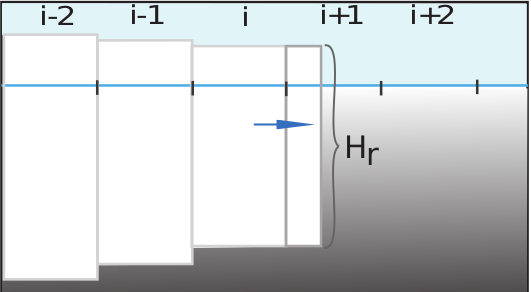
\includegraphics[width=0.7\textwidth,keepaspectratio=true]{Albrechtetal2011half}

\scriptsize volume-of-fluid method at ice shelf fronts

\tiny (Albrecht et al, 2011)

\medskip
\includegraphics[width=0.45\textwidth,keepaspectratio=true]{JaroschSchoofAnslow2013}

\scriptsize glacier ice on steep terrain

\smallskip
\tiny (Jarosch, Schoof, Anslow, 2013)
\end{column}

\begin{column}{0.5\textwidth}
\hfill 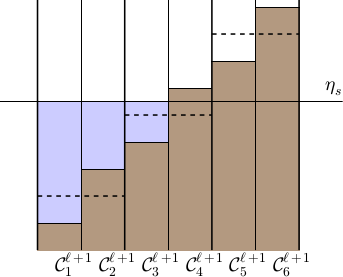
\includegraphics[width=0.45\textwidth,keepaspectratio=true]{LeVequeGeorgeBerger2011}

\hfill \scriptsize tsunami run-up on shore

\smallskip
\hfill \tiny (LeVeque, George, Berger, 2011)

\medskip
\hfill \includegraphics[width=0.55\textwidth,keepaspectratio=true]{jouvet-two-grids}

\hfill \scriptsize volume-of-fluid method at glacier surface

\hfill \tiny (Jouvet et al 2008)
\end{column}
\end{columns}
\end{frame}


\section{Practical conclusions:}

\subsection{approach I: semi-discretize in time}

\begin{frame}{Approach I: semi-discretize in time}

$$h_t + \Div\bq = f \qquad \to \qquad \frac{H_n - H_{n-1}}{\Delta t} + \Div \bQ_n = F_n$$

  \begin{itemize}
  \item semi-discretize in time: $H_n(x) \approx h(t_n,x)$
  \item the new equation is strong form \alert{single time-step problem}
    \begin{itemize}
    \item[$\circ$] a PDE in space where $H_n>0$
    \item[$\circ$] details of flux $\bQ_n$ and source $F_n$ come from time-stepping scheme
      \begin{itemize}
      \item e.g.~$\theta$-methods or RK
      \end{itemize}
    \end{itemize}
  \end{itemize}
\end{frame}


\begin{frame}{1D time-stepping examples (and my $\bq$-agnosticism)}

\begin{columns}
\begin{column}{0.35\textwidth}
\alert{same:}

\begin{itemize}
\scriptsize
\item equation

\tiny
\hspace{-10mm} $\frac{H_n-H_{n-1}}{\Delta t} + \Div\bQ_n = f$
\scriptsize

\item BEuler time-step
\item climate $f$
\item bed shape
\item constraint-respecting

Newton scheme
\end{itemize}

\vspace{2mm}

\alert{top:}

\scriptsize

\medskip
$\bQ_n = v_0 H_n$

hyperbolic advection with

constant velocity

\vspace{5mm}

\normalsize 

\alert{bottom:}

\scriptsize

\medskip
$\bQ_n = - \Gamma |H_n|^{n+2}$

$\phantom{bQ_n = }\, \cdot |\grad s_n|^{n-1} \grad s_n$

nonlinear degenerate

diffusion
\end{column}
\begin{column}{0.55\textwidth}
\hspace{-15mm}
\animategraphics[autoplay,loop,height=3.5cm]{6}{anim/adv/u-}{1}{50}

\medskip
\hspace{-15mm}
\animategraphics[autoplay,loop,height=3.5cm]{6}{anim/sia/u-}{1}{50}
\end{column}
\end{columns}
\end{frame}


\subsection{approach II: each time-step is weakly-posed free-bdry problem}

\begin{frame}{Approach II: weak form incorporates $H_n\ge 0$ constraint}

  \begin{itemize}
  \item define:
    $$\mathcal{K} = \left\{v \in W^{1,p}(\Omega) \,\Big|\, v\ge 0\right\} = \text{\alert{admissible thicknesses}}$$
  \item we say $H_n \in \mathcal{K}$ solves the \alert{weak single time-step problem} if
    $$\int_\Omega H_n (v - H_n) - \Delta t\, \bQ_n \cdot \grad(v - H_n) \ge \int_\Omega \left(H_{n-1} + \Delta t\, F_n\right) (v - H_n)$$
  for all $v \in \mathcal{K}$
  \small
  \medskip
    \begin{itemize}
    \item[$\circ$] derive this \emph{variational inequality} (VI) from:
      \begin{itemize}
      \item[$\diamond$] integration-by-parts on strong form
      \item[$\diamond$] thought about $H_n=0$ areas
      \end{itemize}
    \end{itemize}
  \end{itemize}
\end{frame}


\begin{frame}{Weak solves strong; gives more info}

\begin{itemize}
  \item assume $\bQ_n=0$ when $H_n=0$
    \begin{itemize}
    \item[$\circ$] this means $\bQ_n$ describes a \emph{layer}
    \end{itemize}
  \item if $H_n \in \mathcal{K}$ solves weak single time-step problem (VI) then
  
      \medskip
	  \begin{itemize}
	  \item[$\circ$] PDE applies on the set where $H_n>0$ (interior condition):
	    $$\frac{H_n - H_{n-1}}{\Delta t} + \Div \bQ_n = F_n$$
	  \item[$\circ$] plus inequality on the set where $H_n = 0$:
	    $$H_{n-1} + \Delta t\, F_n \le 0$$
	    \vspace{-6mm}
	    \begin{itemize}
	    \item ``climate negative enough during time step to remove old thickness''
	    \end{itemize}
	  \end{itemize}
\end{itemize}
\end{frame}


\begin{frame}{Alternative weak formulation: NCP}

\begin{itemize}
\item NCP = nonlinear complementarity problem
\item abstractly, NCP is:
  \begin{itemize}
  \item[$\circ$]  given differentiable map $\bF:\RR^n \to \RR^n$
  \item[$\circ$]  solve
     $$\bx \ge 0, \quad \bF(\bx) \ge 0, \quad \bx^\top \bF(\bx) = 0$$
  \end{itemize}
\item our case:
  \begin{itemize}
  \item[$\circ$]  $\infty$ dimensions with m.c.~equation $h_t + \Div\bq = f$
  \item[$\circ$]  $\bx = H_n$ and $\bF(\bx) = (\text{residual from discrete-time m.c.~eqn.})$
  \end{itemize}
\item in finite dimensions we have VI $\leftrightarrow$ NCP equivalence:
  $$\ip{\bF(\bx)}{\by-\bx} \ge 0 \quad \forall \by \in \mathcal{K} \qquad \iff \qquad \text{NCP}$$
\end{itemize}
\end{frame}


\subsection{newly-available numerical tools}

\begin{frame}{Numerical solution of the weak problem}

the weak single time-step problem:
\begin{itemize}
\item is nonlinear because of constraint (even for $\bQ_n$ linear in $H_n$)
\item can be solved by a Newton method modified for constraint
\item scalable implementations are in PETSc$^*$ 3.5+
  \begin{itemize}
  \item[$\circ$]  see ``SNESVI'' object
  \item[$\circ$]  for NCP there are two implementations (Benson \& Munson, 2006):
    \begin{itemize}
    \item  reduced-set (active-set) method
    \item  semismooth method
    \end{itemize}
  \end{itemize}
\end{itemize}

\vspace{15mm}
{\scriptsize $^*$Portable Extensible Toolkit for Scientific computation, \texttt{www.mcs.anl.gov/petsc}}
\end{frame}


\begin{frame}{Example: Greenland ice sheet}

\begin{columns}
\begin{column}{0.6\textwidth}
\begin{itemize}
\small
\item given steady climate and bedrock elevations, what is shape of Greenland ice sheet?
  \begin{itemize}
  \scriptsize
  \item[$\circ$] climate = ``surface mass balance''
  \item[] \qquad = precipitation $-$ runoff-from-melt
  \end{itemize}
\small
\item assume simplest reasonable dynamics: non-sliding shallow ice approximation
\item solve VI/NCP weak problem
  \begin{itemize}
  \scriptsize
  \item[$\circ$] steady state ($\Delta t\to \infty$)
  \item[$\circ$] reduced-set Newton method
  \item[$\circ$] 900 m structured grid
  \item[$\circ$] $Q^1$ FEs in space
  \item[$\circ$] $N=7\times 10^6$ d.o.f.
  \end{itemize}
\end{itemize}

\vspace{5mm}
\tiny (Bueler, submitted to J.~Glaciol.)
\end{column}
\begin{column}{0.4\textwidth}
\vspace{-5mm}

\begin{center}
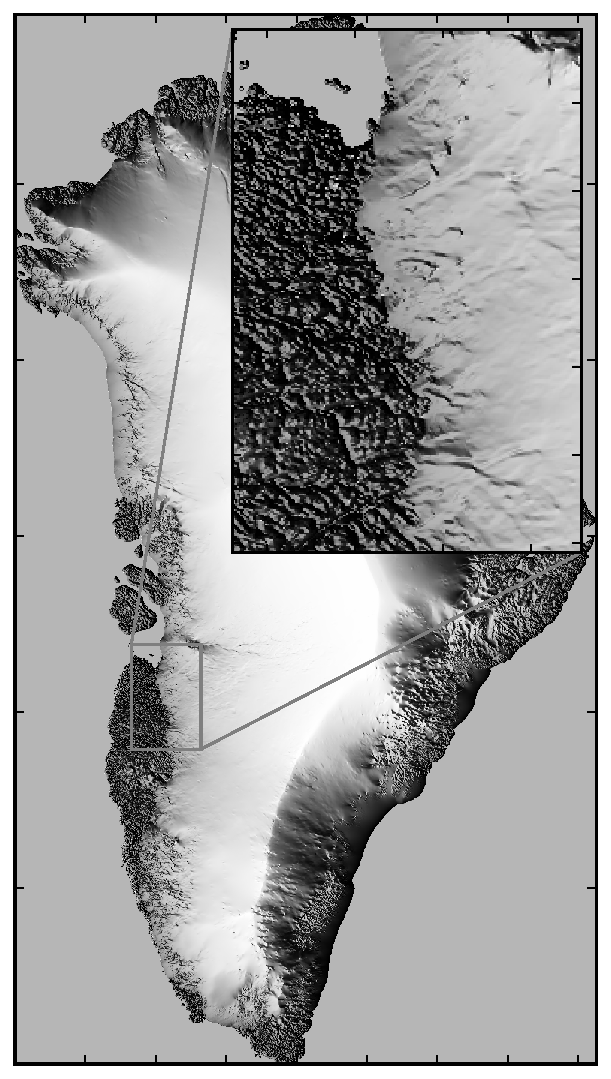
\includegraphics[width=0.95\textwidth,keepaspectratio=true]{grnwinset}
\end{center}
\end{column}
\end{columns}
\end{frame}


\subsection{new (?) limitations to discrete conservation}

\begin{frame}{Conservation reporting: subsets}
\begin{itemize}
\item suppose $H_n$ solves the single time-step problem
\item define
	\begin{align*}
	\Omega_n &= \left\{H_n(x) > 0\right\} \\
	\Omega_n^r &= \left\{H_n(x)= 0 \text{ and } H_{n-1}(x) > 0\right\} \quad \text{\alert{$\leftarrow$ retreat set}}
	\end{align*}
\end{itemize}

\vspace{-3mm}
\begin{center}
\includegraphics[width=0.8\textwidth,keepaspectratio=true]{cartoon-sets}
\end{center}
\end{frame}


\begin{frame}{Conservation reporting: time-series}

\begin{itemize}
\item define:
   $$M_n = \int_\Omega H_n(x)\,dx \qquad \text{\emph{mass at time} $t_n$}$$
\item then \vspace{-5mm}
	\begin{align*}
	M_n - M_{n-1} &= \int_{\Omega_n} \mathLabelBox[
    labelstyle={xshift=1cm,yshift=2mm},
    linestyle={out=270,in=90, -latex}
    ]{H_n - H_{n-1}}{$\boxed{\Delta t\, (-\Div\bQ_n + F_n)}$} \,dx + \int_{\Omega_n^r} 0 - H_{n-1} \,dx \\
	   &= \Delta t\, \left(0 + \int_{\Omega_n} F_n \,dx\right) - \int_{\Omega_n^r} H_{n-1} \,dx
	\end{align*}
\item new term:
     $$R_n = \int_{\Omega_n^r} H_{n-1} \,dx \qquad \text{\emph{\alert{retreat loss} during step} $n$}$$
\end{itemize}
\end{frame}


\begin{frame}{Conservation reporting: \emph{limitation}}

\begin{itemize}
\item \alert{the retreat loss $R_n$ is not balanced by the climate}
  \begin{itemize}
  \item[$\circ$] $R_n$ is \emph{caused} by the climate, but we don't know a computable integral of climate $F_n$ to balance it
  \end{itemize}
\item we must track \alert{three} time series:
  \begin{itemize}
  \item[$\circ$] mass at time $t_n$: \qquad $M_n = \int_\Omega H_n(x)\,dx$

  \smallskip
  \item[$\circ$] climate (e.g.~surface mass bal.) over current fluid-covered region:
     $$C_n = \Delta t\, \int_{\Omega_n} F_n \,dx \qquad \approx \int_{t_{n-1}}^{t_n} \int_{\Omega_n} f(t,x) \,dx\,dt$$
  \item[$\circ$] retreat loss during time step: \qquad $R_n = \int_{\Omega_n^r} H_{n-1} \,dx$
  \end{itemize}
\item now it balances:
     $$M_n = M_{n-1} + C_n - R_n$$
\end{itemize}
\end{frame}


\begin{frame}{Reporting discrete conservation: $R_n\to 0$ as $\Delta t\to 0$}

\begin{center}
\vspace{-3.3mm}

\animategraphics[autoplay,loop,height=2.9cm]{15}{anim/tdep/u-}{1}{250}

\vspace{-1.1mm}
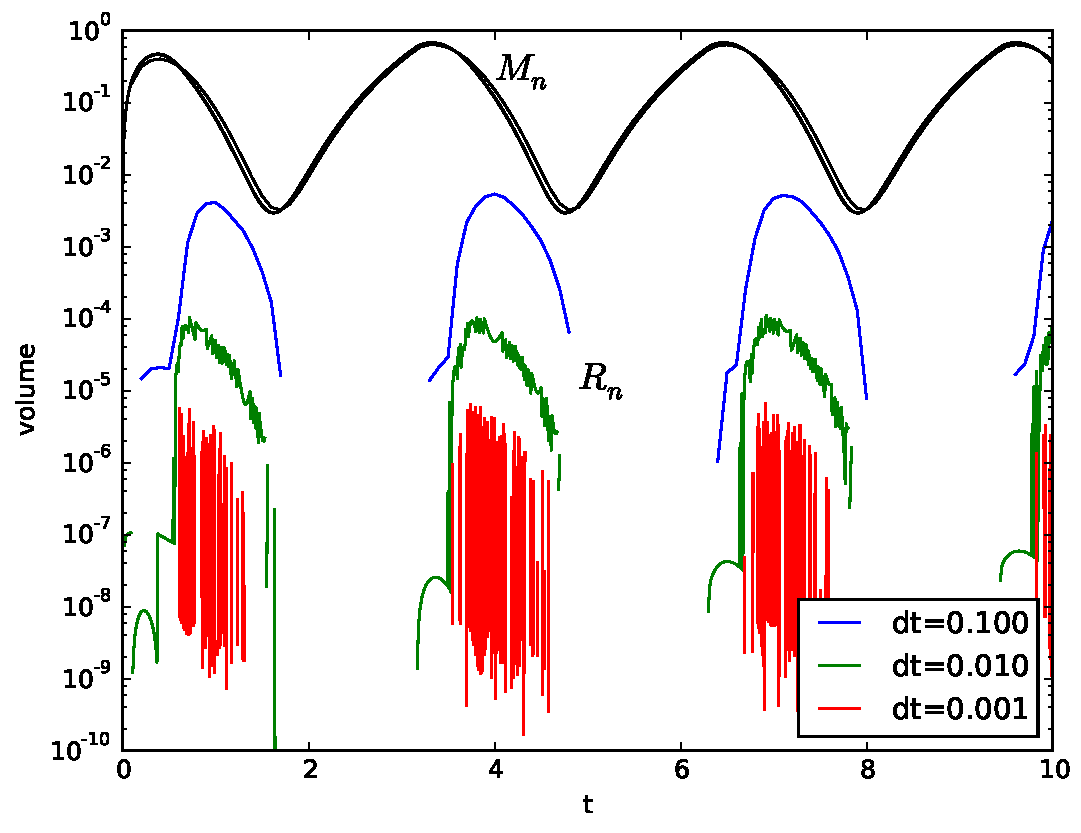
\includegraphics[width=0.59\textwidth,keepaspectratio=true]{masstimeseries} \, \phantom{!}
\end{center}
\end{frame}


\begin{frame}{Summary}

consider layer flow model \, $h_t + \Div\bq = f$ \, subject to signed climate $f$ and where $h$ is layer thickness

  \begin{itemize}
  \item goals/issues:
    \begin{itemize}
    \item[$\circ$]  long time steps wanted
    \item[$\circ$]  models have been limited by free-boundary lack-of-clarity
    \end{itemize}
  \item approach:
    \begin{itemize}
    \item[$\circ$]  include constraint on thickness: $h\ge 0$
    \item[$\circ$]  consider discrete-time problem before doing FEM/FVM/etc.
    \item[$\circ$]  pose single time-step problem weakly as VI or NCP
    \item[$\circ$]  solve by scalable constrained-Newton method (PETSc)
    \end{itemize}
  \item new (?) result:
    \begin{itemize}
    \item[$\circ$]  discrete conservation requires tracking retreat-loss time-series
      \begin{itemize}
      \item in addition to climate input during time step
      \end{itemize}
    \end{itemize}
  \end{itemize}

\end{frame}

\end{document}


